\documentclass{ximera}

\input{../preamble.tex}


\title[Problem 1]{Problem 1}

\begin{document}
\begin{abstract} \end{abstract}
\maketitle


% Extracted from applicationsOfIntegrals.tex, problem #1
\begin{problem}

Solve the following word problems:

	\begin{enumerate}

	\item  The velocity function for an object moving along a line east/west is given by
	$v(t) = -t^2 + 4t - 3$ feet per minute.

		\begin{enumerate}

		\item  Find the total displacement the object traveled from $2$ minutes to $6$ minutes (assume east is positive).
		\begin{explanation}
				The object's total displacement is given by $\displaystyle \int_2^6 v(t) \d t$.  So we compute:
					\begin{align*}
						\displaystyle \int_2^6 v(t) \d t &= \displaystyle \int_2^6 (-t^2 + 4t - 3) \d t  \\
							&= \eval{- \dfrac{1}{3} t^3 + 2t^2 - 3t}_2^6  \\
							&= (-72 + 72 - 18) - \left( - \dfrac{8}{3} + 8 - 6 \right)  \\
							&= \dfrac{8}{3} - 20 = - \dfrac{52}{3}.
						\end{align*}
				So the object's displacement is $\dfrac{52}{3}$ feet west of its original location.
			\end{explanation}

		\item  Find the total distance the object traveled from $2$ minutes to $6$ minutes.
		\begin{explanation}
				First notice that $v(t) = -(t^2 - 4t + 3) = -(t-1)(t-3)$.  So we can see that
					\begin{align*}
						v(t) &> 0 \text{ when }  2 \leq t < 3.  \\
						v(t) &< 0 \text{ when } 3 < t \leq 6.
					\end{align*}
					Thus, the total distance that the object traveled from $2$ minutes to $6$ minutes is:
					\begin{align*}
						\displaystyle \int_2^6 \left| v(t) \right| \d t &= \displaystyle \int_2^3 \left| v(t) \right| \d t + \displaystyle \int_3^6 \left| v(t) \right| \d t  \\
							&= \displaystyle \int_2^3 v(t) \d t + \displaystyle \int_3^6 - v(t) \d t  \\
							&= \displaystyle \int_2^3 (-t^2 + 4t - 3) \d t - \displaystyle \int_3^6 (-t^2 + 4t - 3) \d t  \\
							&= \eval{- \dfrac{1}{3} t^3 + 2t^2 - 3t}_2^3 - \eval{- \dfrac{1}{3} t^3 + 2t^2 - 3t}_3^6  \\
							&= \left( (-9+18-9) - (- \dfrac{8}{3} + 8 - 6) \right) -  \\
							& \left( (-72+72-18)-(-9+18-9) \right)  \\
							&= \left(0 - 2 + \dfrac{8}{3} \right) - \left( -18 - 0 \right)  \\
							&=  16 + \dfrac{8}{3} = \dfrac{56}{3}.
					\end{align*}
				So, the total distance that the object traveled is $\dfrac{56}{3}$ feet.
			\end{explanation}

		\item  Suppose that the object's position $2$ minutes into the trip is $5$ feet of a placement marker.  What is its position (relative to the placement marker) at $6$ minutes.
		\begin{explanation}
				$s(6) = s(2) + \displaystyle \int_2^6 v(t) \d t = 5 + \left(- \dfrac{52}{3} \right) = - \dfrac{37}{3}. $

				So the object's position at $6$ minutes is $\dfrac{37}{3}$ feet west of the placement marker.
			\end{explanation}
		\end{enumerate}
		
		\item  Sammy the Snail sets up camp in the median of I-70 and, starting at noon and ending at 6pm, hikes back and forth along the highway.  He starts his hike at his campsite.  His velocity at time $t$ hours (after noon)  is given by $v(t)=(t-2)(t-5)$ inches per hour.  Find the total distance Sammy travelled on his hike.
		\begin{explanation}
			The total distance that Sammy travels is $\displaystyle \int_0^6 \left| v(t) \right| \d t$.
			The following picture indicates where $v(t)$ is positive and negative:
				\begin{image}
				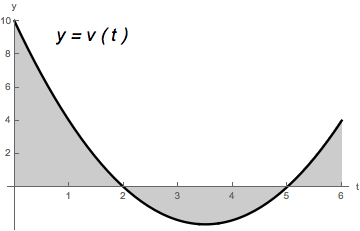
\includegraphics{figure16.png}
				\end{image}
				So we compute:
				\begin{align*}
					\displaystyle \int_0^6 \left| v(t) \right| \d t &= \displaystyle \int_0^2 \left| v(t) \right| \d t + \displaystyle \int_2^5 \left| v(t) \right| \d t + \displaystyle \int_5^6 \left| v(t) \right| \d t  \\
						&= \displaystyle \int_0^2 v(t) \d t - \displaystyle \int_2^5 v(t) \d t + \displaystyle \int_5^6 v(t) \d t  \\
						&= \displaystyle \int_0^2 (t^2 - 7t + 10) \d t - \displaystyle \int_2^5 (t^2 - 7t + 10) \d t + \displaystyle \int_5^6 (t^2 - 7t + 10) \d t  \\
						&= \eval{\dfrac{1}{3}t^3-\dfrac{7}{2}t^2+10t}_0^2-\eval{\dfrac{1}{3}t^3-\dfrac{7}{2}t^2+10t}_2^5+\eval{\dfrac{1}{3}t^3-\dfrac{7}{2}t^2+10t}_5^6  \\
						&= \left( \left(\dfrac{8}{3}-14+20 \right)-0\right)-\left( \left( \dfrac{125}{3}-\dfrac{175}{2}+50 \right)-\left( \dfrac{8}{3}+6 \right) \right)+  \\
						&\left( \left( 72-126+60 \right) - \left( \dfrac{125}{3} - \dfrac{175}{2} + 50 \right) \right)  \\
						&= -82+175-78=15.
				\end{align*}
			So Sammy has traveled a distance of $15$ inches.
		\end{explanation}
	\end{enumerate}
\end{problem}



\end{document}
